\section{Reference model for Open Source Software Processes Discovery}
Jensen \& Scacchi in \cite{citeulike:5043664} are taking a somewhat different approach from previously discussed. Authors are following a top-down approach and not trying to build a software process model from available process artifacts but rather trying to revise an existing software process \textit{reference model} by iteratively refining mapping between observed artifacts and the model entities. 

The proposed by authors, software process \textit{reference model}, is a layer which provides a mapping from the underlying recognized software process artifacts into a higher level software-process meta-model by Mi \& Sacchi \cite{citeulike:5128872}. The iterative revision of the reference model vocabulary of mapped terms (Figure \ref{fig:refterm}) is performed through the case studies. During such a study, the observed process artifacts such as SCM logs, defect reports and others are queried with terms from the reference model pulling correlated artifacts which are revised and curated by the process expert and lead to the further revisions of the terms taxonomy on the next iteration.

\begin{figure}[tbp]
   \centering
   \includegraphics[height=40mm]{refterm.eps}
   \caption{Example of the reference model mapping from \cite{citeulike:5043664}.}
   \label{fig:refterm}
\end{figure}

The use of a created in such an iterative fashion reference model provides an experience and certain assurance in the research of the novel process which was the aim of the authors. 

As per applicability of such a methodology to my research, I am envisioning the creation of the software process low-level patterns taxonomy which might be helpful in the understanding of the phenomena behind observed unknown recurrent behavior.
